\documentclass[a4paper]{scrbook}

\usepackage[utf8]{inputenc}
\usepackage{graphicx}
\usepackage{booktabs}
\usepackage{url}
\usepackage{relsize}
\usepackage{hyperref}
\usepackage{libertine}
\usepackage{ifthen}
% \usepackage{fancyhdr}
% \KOMAoptions{open=any}


%%%%%%%%%%%%%%%%%%%%%%%%%%%%%%%%%%%%%%%%%%%%%%%%%%%%%%%%%%%%%%%%%%%%%%%%%%%%%%%%
% Replace these values
%%%%%%%%%%%%%%%%%%%%%%%%%%%%%%%%%%%%%%%%%%%%%%%%%%%%%%%%%%%%%%%%%%%%%%%%%%%%%%%%
\newcommand{\thesistitleDE}{Erzeugung optischer Fernerkundungsdaten (Sentinel-2) auf Basis von Radar-Fernerkundungsdaten (Sentinel-1) mittels generativer KI}
\newcommand{\thesistitleEN}{Generation of optical remote sensing data (Sentinel-2) based on radar remote sensing data (Sentinel-1) using generative AI}

\newcommand{\student}{Ahmed Attia}
\newcommand{\matrnr}{00815907}
\newcommand{\stammnr}{} % Unset this variable if you only have a (single) matriculation number
% \newcommand{\stammnr}{234567} % Unset this variable if you only have a (single) matriculation number
\newcommand{\submissiondate}{XX.\ Monat 20XX}
\newcommand{\supervisor}{Dr. Peter Hofmann}
\newcommand{\secsupervisor}{} % Unset this variable if no second supervisor is required
% \newcommand{\secsupervisor}{Prof.~Dr.~Zweitprüfer} % Unset this variable if no second supervisor is required
\newcommand{\faculty}{Angewandte Informatik}

% Select your course of studies here
\newcommand{\studies}{Bachelor Künstliche Intelligenz}
\newcommand{\degree}{Bachelor of Science (B.Sc.)}
%%%%%%%%%%%%%%%%%%%%%%%%%%%%%%%%%%%%%%%%%%%%%%%%%%%%%%%%%%%%%%%%%%%%%%%%%%%%%%%%

\renewcommand*{\UrlFont}{\ttfamily\smaller\relax}

\begin{document}
\pagestyle{headings}
\pagenumbering{roman}


\setkomafont{title}{\Large \scshape}
\begin{titlepage}
\begin{center}
	{\usekomafont{subject}
	Technische Hochschule Deggendorf\\
	Fakultät \faculty\par}
	\vspace{.2cm}
{\Large \studies\\}
% {\Large Studiengang \studies\\}
\vspace{6\baselineskip}
{\usekomafont{title}\thesistitleDE\par}
\vspace{1cm}
{\usekomafont{title}\thesistitleEN\par}
\vspace{6\baselineskip}

\usekomafont{publishers}
Bachelorarbeit zur Erlangung des akademischen Grades:
% Masterarbeit zur Erlangung des akademischen Grades:

	\vspace{.2cm}
	\emph{\degree}
	\vspace{.2cm}

an der Technischen Hochschule Deggendorf\\
\end{center}
\vfill
\parbox[t]{.4\textwidth}{\usekomafont{author}
	Vorgelegt von:\\
	\student\\
	Matrikelnummer: \matrnr\par
	\ifthenelse{\equal{\stammnr}{}}{}{
	Stammnummer: \stammnr\par
	}
	\vspace{\baselineskip}
	Am: \submissiondate\par
}
\hfill
\parbox[t]{.4\textwidth}{\usekomafont{author}
Prüfungsleitung:\\
\supervisor%

\ifthenelse{\equal{\secsupervisor}{}}{}
{%
\vspace{\baselineskip}
Ergänzende Prüfende:\\
\secsupervisor%
}}
\end{titlepage}
\cleardoublepage\par
% \clearpage\par
% Erklärung über die Selbständigkeit der Arbeit
\thispagestyle{empty}
\newcommand{\signature}[1]{%
\bigskip
\noindent
\begin{tabular*}{\linewidth}{lp{3cm}p{1cm} p{6cm}}
Deggendorf, & \dotfill & & \dotfill \\
& {\footnotesize Datum} & & {\centering \footnotesize #1}
\end{tabular*}
}

\begin{minipage}[b]{.5\linewidth}
	\Large\textbf{Erklärung}
\end{minipage}
\begin{minipage}[b]{.5\linewidth}
	
\includegraphics[width=\linewidth]{img/THD_Logo.pdf}
\end{minipage}

\bigskip

Name des Studierenden: \quad \student

\bigskip
Name des Betreuenden: \quad \supervisor

\vspace{.7cm}
Thema der Abschlussarbeit:

\vspace{.5em}
{\def\\{\relax\ifhmode\unskip\fi\space\ignorespaces}
\thesistitleDE
}\dotfill

\vspace{.5em}
\dotfill

\vspace{.5em}
\dotfill

\vspace{.5em}
\dotfill

\begin{enumerate}
	\item Ich erkläre hiermit, dass ich die Abschlussarbeit gemäß § 35 Abs.~7 RaPO (Rahmen\-prüf\-ungs\-ordnung für die Fachhochschulen in Bayern, BayRS 2210-4-1-4-1-WFK)  selbständig  verfasst,  noch  nicht  anderweitig  für Prüfungszwecke  vorgelegt,  keine  anderen  als  die  angegebenen  Quellen  oder Hilfsmittel  benutzt  sowie  wörtliche  und  sinngemäße  Zitate  als  solche gekenn\-zeichnet habe.

		\signature{Unterschrift des Studierenden}

	\item  Ich  bin  damit  einverstanden, dass die von  mir angefertigte  Abschlussarbeit über die Bibliothek der Hochschule einer breiteren Öffentlichkeit zugänglich gemacht wird:
		\begin{itemize}
			\item[$\bigcirc$] Nein
			\item[$\bigcirc$] Ja, nach Abschluss des Prüfungsverfahrens
			\item[$\bigcirc$] Ja, nach Ablauf einer Sperrfrist von \ldots Jahren.
		\end{itemize}

		\signature{Unterschrift des Studierenden}
\end{enumerate}

\noindent
\hrulefill

{\centering{\footnotesize Bei Einverständnis des Verfassenden vom Betreuenden auszufüllen:}}

{\flushleft

Eine Aufnahme eines Exemplars der Abschlussarbeit in den Bestand der Bibliothek und die Ausleihe des Exemplars wird:

\begin{itemize}
	\item[$\bigcirc$] Befürwortet
	\item[$\bigcirc$] Nicht befürwortet
\end{itemize}

		\signature{Unterschrift des Betreuenden}
}

% \cleardoublepage\par
\clearpage


\chapter*{Abstract}
\addcontentsline{toc}{chapter}{Abstract}


\tableofcontents
\cleardoublepage

\setcounter{page}{1}
\pagenumbering{arabic}


\chapter{Introduction}

Earth observation has become an indispensable tool for understanding and monitoring the planet’s dynamic processes. Optical and radar remote sensing represent two complementary modalities at the core of modern Earth observation systems. Optical sensors provide rich spectral and visual information suitable for human interpretation. This information is used, among others, in forest prediction, agricultural monitoring, military, etc~\cite{S2MS_GAN}. However, they are inherently constrained by atmospheric conditions such illumination variability and in particular cloud cover. This causes considerable data gaps in both the spatial and temporal domains~\cite{CR_SEN2_dRNN}. 
In contrast, synthetic aperture radar (SAR) sensors operate in the microwave domain, offering all-weather, day-and-night imaging capabilities independent of sunlight or cloud interference. However, the backscatter-based nature of SAR imagery introduces challenges related to speckle noise, geometric distortions, and the absence of spectral color information~\cite{bench_sar_color, naderi2021}, complicating its interpretation.

To bridge the gap between these two sensing modalities, SAR-to-optical image translation has emerged as a powerful generative approach. It aims to synthesize optical-like, cloud-free imagery from SAR data, combining the interpretability of optical observations with the robustness of radar acquisitions. Recent advances in generative artificial intelligence (GenAI), particularly in conditional generative adversarial networks (cGANs) and diffusion models, have made it possible to learn complex mappings between SAR and optical domains with remarkable realism~\cite{cr_fuse_HR_GEN}. 
These developments have opened new pathways for applications in land-cover classification, vegetation monitoring, disaster response, and particularly, cloud removal. % keep or delete?

Despite the rapid progress in this field, most existing studies have focused primarily on reconstructing the visible RGB subset of optical imagery, with a few extending to the NIR range, leaving the full multispectral potential of missions such as Sentinel-2 largely underexplored. Furthermore, while SAR-to-optical translation is often evaluated qualitatively, systematic assessments of its reliability across individual spectral bands remain limited. Finally, although the approach shows promise for cloud removal, its effectiveness in this context has not yet been comprehensively validated across the full spectral range

Against this background, the present thesis investigates the use of generative models for translating Sentinel-1 SAR imagery into multispectral Sentinel-2 optical data. The work is guided by three main objectives:
\begin{enumerate}
    \item To validate SAR-to-optical image translation across the full 13 Sentinel-2 spectral bands. 
    \item To assess how reliably each optical band can be individually reconstructed and to what extent.
    \item To evaluate the performance of SAR-to-optical image translation for cloud removal
\end{enumerate}

Through these objectives, this thesis aims to provide a comprehensive and quantitative understanding of SAR-to-optical translation as a multimodal learning problem, highlighting its strengths, limitations, and potential for operational cloud-free optical data generation.

\bigskip
\textcolor{red}{layout the thesis}
% \noindent
% \textbf{Thesis Structure.}
The remainder of this thesis is organized into six chapters, each addressing a distinct component of the research.
Chapter~\ref{ch:background} provides the theoretical background and literature review, introducing the fundamentals of remote sensing, the Copernicus Sentinel missions, cloud removal methodologies, and generative artificial intelligence for multimodal data fusion.
Chapter~\ref{ch:methodology} outlines the methodological framework, including the problem formulation, dataset selection, preprocessing pipeline, and the design of the \textit{Pix2Pix} model together with its training and evaluation procedures.
Chapter~\ref{ch:results} presents the experimental results and analyses, covering the main evaluation scenarios: reconstruction on partial and full datasets, per-band performance assessment, and validation on cloud removal tasks.
Chapter~\ref{ch:ablation} reports the ablation studies that examine the effect of different loss functions and the exclusion of specific spectral bands, providing a deeper understanding of the model’s behavior.
Chapter~\ref{ch:challenges} discusses the main challenges encountered during experimentation, such as training instability and artifact formation, along with the corrective strategies implemented.
Finally, Chapter~\ref{ch:limitations} concludes the work by summarizing its limitations and outlining future research directions, including temporally generalized learning, diffusion-based architectures, and band-aware normalization strategies.
Supplementary material, such as per-band reconstructions and seasonal evaluations, is included in the appendices.

The remainder of this thesis is organized as follows.
Chapter~\ref{ch:background} introduces the theoretical background, including remote sensing fundamentals, the Sentinel missions, cloud removal methods, and generative AI approaches.
Chapter~\ref{ch:methodology} describes the methodological framework, dataset preparation, and the adopted Pix2Pix model.
Chapter~\ref{ch:results} presents the experimental results and evaluation across multispectral reconstruction and cloud removal tasks.
Chapter~\ref{ch:ablation} reports the ablation studies investigating the effect of different loss configurations and band exclusions.
Chapter~\ref{ch:challenges} discusses the challenges encountered during model training and their mitigation.
Finally, Chapter~\ref{ch:limitations} summarizes the limitations, draws conclusions, and outlines directions for future research.
\chapter{Background}

\section{Remote Sensing}
Remote sensing (RS) is commonly defined as the acquisition of information about an object through sensors without direct physical contact. This information is obtained by detecting and measuring the modifications the object induces in its surrounding fields, which may include electromagnetic, acoustic, or potential fields \cite{book_Physics_Techniques_RS}.

RS is a relatively recent scientific discipline characterized by its strong interdisciplinary nature. It draws upon a wide spectrum of fields, requiring practitioners to develop a broad foundational understanding of both natural and applied sciences. Effective research in remote sensing often involves collaboration with specialists in electromagnetic theory, spectroscopy, applied physics, geology, atmospheric sciences, oceanography, electrical engineering, and optical engineering \cite{book_Physics_Techniques_RS}.

Remote observations require an interaction of energy between the target and the sensor. In the case of passive sensors, the detected energy originates from external or natural sources, such as solar radiation reflected by the Earth's surface or thermal radiation emitted by the object itself. A prominent example is the \textit{Landsat} program \footnote{https://landsat.gsfc.nasa.gov/}, which represents the longest continuously operating Earth observation mission. Over several decades, Landsat has generated a continuous global record, contributing significantly to environmental monitoring and Earth system science.

By contrast, active sensors generate their own energy pulses to illuminate the target and subsequently measure the portion of the signal that is reflected or backscattered. This capability allows them to operate independently of solar illumination and under a wide range of environmental conditions, including day or night and, in the case of microwave systems, through cloud cover and adverse weather \cite{RS_platforms_survey}. The most widely used active sensing technologies are Radar (Radio Detection and Ranging), which transmits and receives microwave radiation, and LiDAR (Light Detection and Ranging), which employs laser pulses in the optical domain. Both systems record the properties of the reflected signals to extract information about the target.

The term \textit{Remote Sensing} was introduced in the early 1960s to denote techniques for observing the Earth from a distance, with particular reference to aerial photography, which represented the predominant sensing technology at that time \cite{book_Satellite_RS}.

With the advent of satellites, global and synoptic observations of Earth and other planetary environments have become possible. Earth-orbiting sensors provide essential data on atmospheric dynamics, cloud distribution, vegetation cover, and its seasonal variability. Their long-term operation and repetitive coverage enable the monitoring of rapidly changing processes, such as polar ice dynamics and tropical deforestation. Beyond Earth, planetary missions (orbiters, flybys, landers, and rovers) have extended similar observations to all major planets in the solar system. To date, every planet has been visited at least once \cite{book_Physics_Techniques_RS}.
% \newpage

The origins of remote sensing date back to the invention of photography in 1839, which soon after was applied to topographic mapping. By the mid-19th century, aerial photographs were obtained from balloons, followed later by kites, pigeons, and eventually airplanes—the latter marking a decisive step with Wilbur Wright's first aerial photographs in 1909. Aerial photography became essential during World War I and advanced further in the 1930s-1940s with the introduction of color and infrared-sensitive films, widely used during World War II for reconnaissance and camouflage detection \cite{book_Physics_Techniques_RS,book_Satellite_RS}.

\begin{figure}[H]
  \centering
  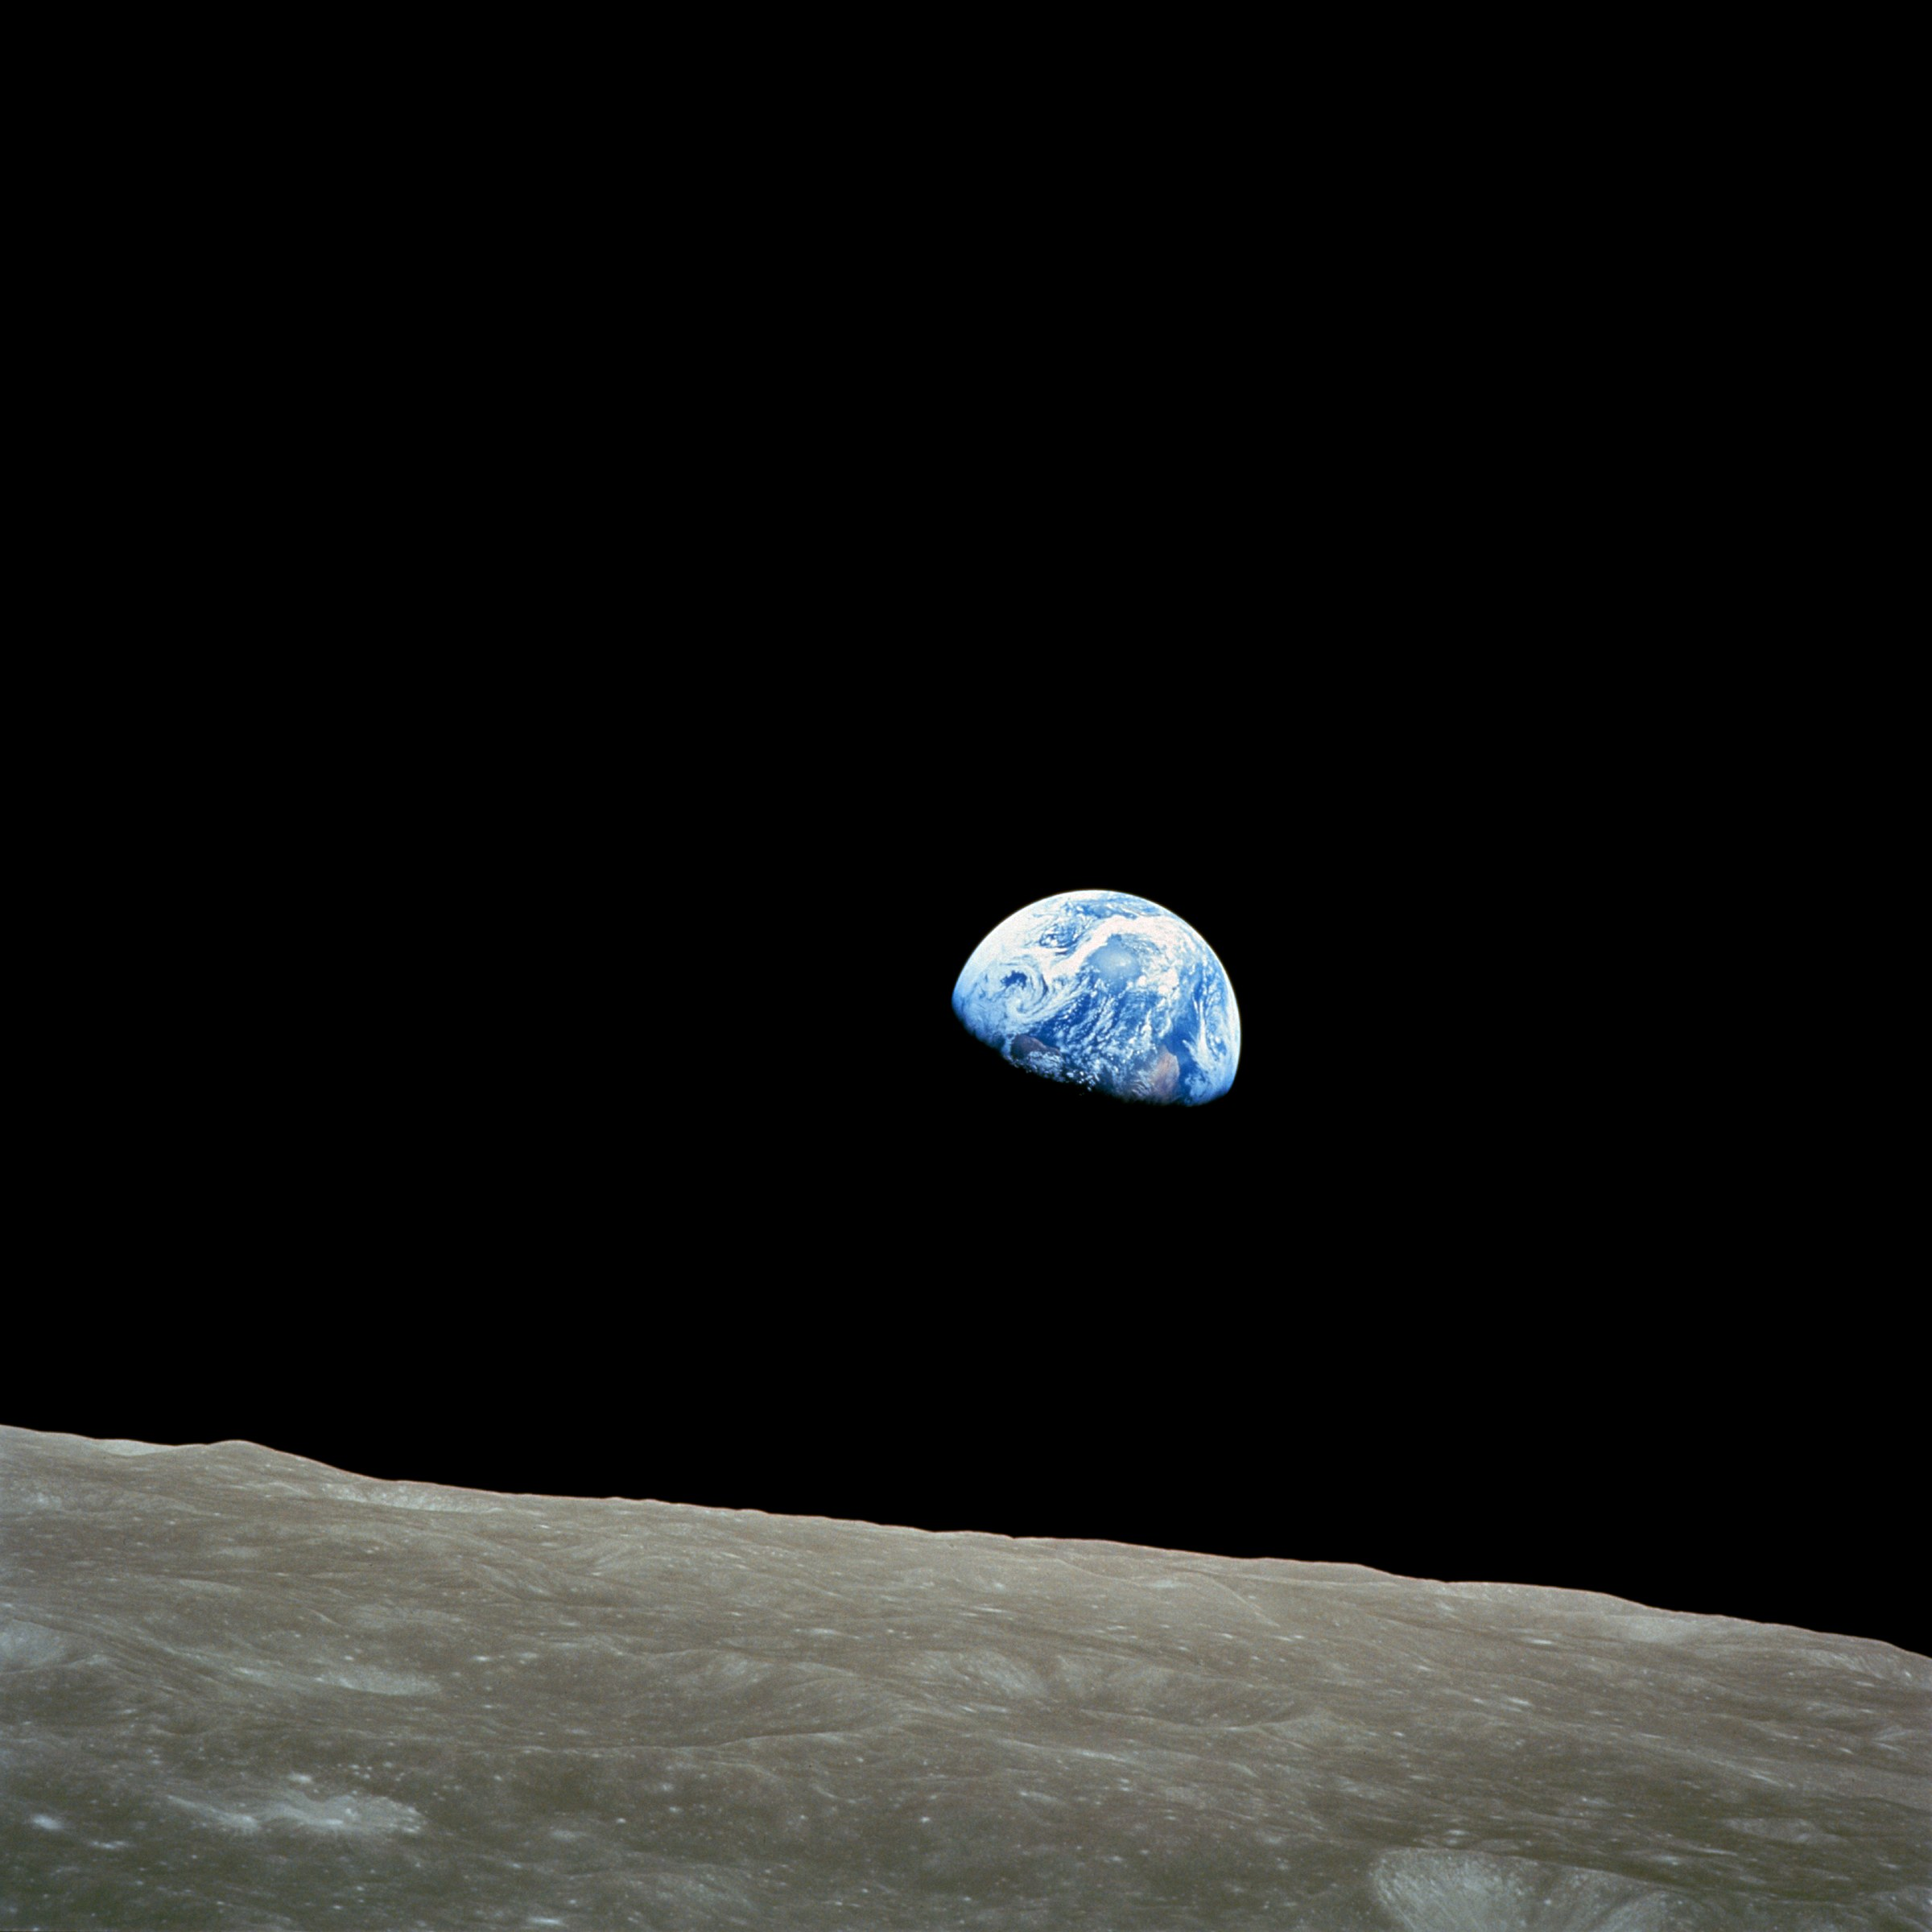
\includegraphics[width=0.95\textwidth]{img/earthrise.jpg}
  \caption{The iconic “Earthrise” photograph taken by astronaut William Anders during the Apollo 8 mission in 1968. Source: NASA.}
  \label{fig:earthrise}
\end{figure}

The postwar decades brought rapid technological progress with the development of radar and synthetic aperture radar (SAR), enabling high-resolution imaging independent of daylight or weather. Early rocket experiments in the late 1940s foreshadowed the space age, initiated by the launch of Sputnik in 1957. NASA's TIROS-1 satellite (1960) delivered the first global meteorological observations, while the launch of Landsat-1 in 1972 introduced systematic multispectral Earth observation, a program that continues today as the longest-running record of land surface change \cite{book_Physics_Techniques_RS,book_Satellite_RS}.

A symbolic milestone came with the Apollo 8 mission in 1968, when astronaut William Anders captured the famous Earthrise photograph, showing Earth rising above the lunar horizon (see Figure \ref{fig:earthrise}). This image not only had profound cultural, philosophical, and scientific impact but also highlighted the scientific value of spaceborne Earth observation.

Since the 1980s, remote sensing has expanded through international efforts such as SPOT (France, 1986), MOS-1 (Japan, 1987), and IRS-1 (India, 1988). The European Space Agency (ESA) \footnote{https://www.esa.int/} launched its first radar satellite, ERS-1, in 1991, and a second with comparable specifications in 1995. The 1990s and 2000s saw the rise of commercial satellites like IKONOS and QuickBird, offering very high-resolution imagery. Today, constellations of small satellites operated by private companies provide near-daily global coverage at meter-scale resolution. These advances—driven by improvements in optics, sensors, data transmission, and digital processing—have transformed remote sensing into a cornerstone of Earth system science, environmental monitoring, disaster response, and planetary exploration \cite{book_Satellite_RS}.

A summary of major milestones in the historical development of remote sensing platforms, from early balloon photography to modern satellite constellations, is illustrated in Figure~\ref{fig:RS_timeline}.

\begin{figure}[H]
  \centering
  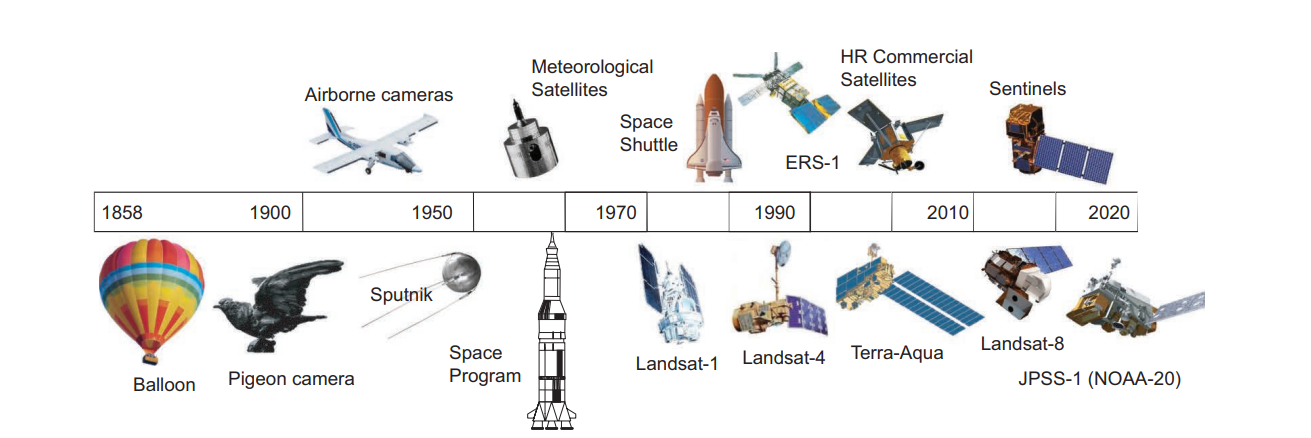
\includegraphics[width=\textwidth]{img/RS_timeline.png}
  \caption{Timeline of remote sensing platform development, from early airborne cameras to modern Earth observation satellites. Adapted from \cite{book_Satellite_RS}.}
  \label{fig:RS_timeline}
\end{figure}


\section{Copernicus: Europe's eyes on Earth}
Copernicus, known as the most ambitious Earth observation programme, is the Earth observation component of the European Union's Space Programme.
It is funded, coordinated, and managed by the European Commission in cooperation with partners such as the European Space Agency (ESA) and the European Organisation for the Exploitation of Meteorological Satellites (EUMETSAT)\footnote{https://www.eumetsat.int/}. The programme was named after the European scientist and observer Nicolaus Copernicus\footnote{https://www.biography.com/scientists/nicolaus-copernicus}. It integrates satellite and in situ observations (e.g., ground stations, airborne and seaborne instruments) to provide reliable, up-to-date information. Its services cover six domains: land, marine, atmosphere, emergency management, security, and climate change. 

The Copernicus Space Component features a new family of dedicated satellites,
called Sentinels, depicted in Figure \ref{fig:sentinels}, specifically designed for the operational needs of the Copernicus programme. 

\begin{figure}[H]
  \centering
  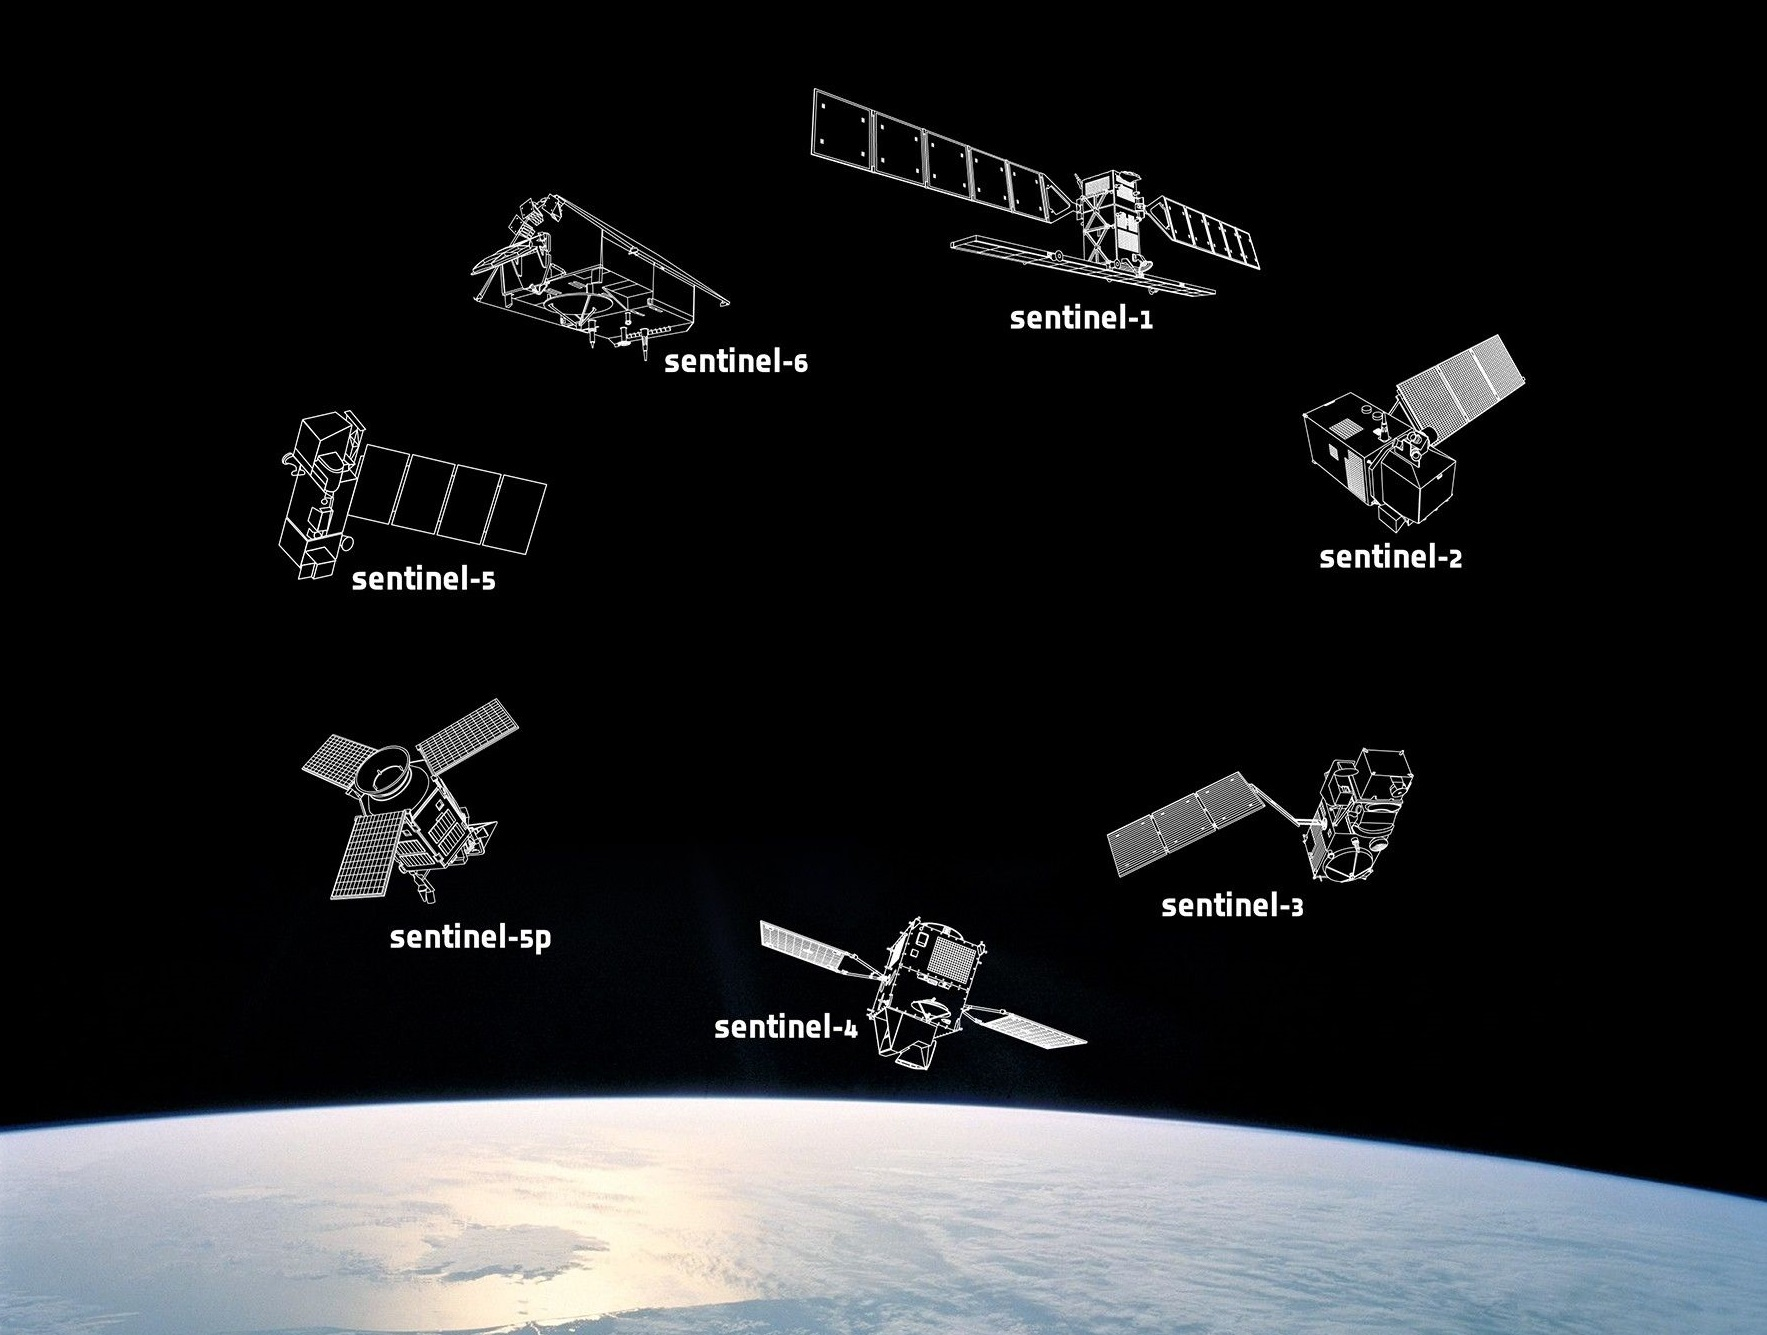
\includegraphics[width=0.95\textwidth]{img/sentinels.png}
  \caption{An artist's impression of the Copernicus Sentinel Missions. Source: ESA.}
  \label{fig:sentinels}
\end{figure}

On 3 April 2014, the deployment of the Copernicus Space Component began with the
launch of the \textsc{Sentinel-1} radar satellite, operating in the C-band and providing all-weather, day-and-night radar imagery. It was followed by its radar successors in 2016 and 2024. Its synthetic aperture radar (SAR) instruments are crucial for monitoring land deformation, subsidence, sea-ice dynamics, and emergency situations such as flooding and earthquakes \cite{ESA_Copernicus,ESA_SentinelMissions}.

\textsc{Sentinel-2}, launched in 2015, 2017, and 2024, is designed to deliver high-resolution, multispectral optical images, supporting applications such as agriculture, forestry, land use, disaster management, and climate studies. Its 13 spectral bands enable detailed analysis of vegetation health, water quality, and land cover dynamics \cite{ESA_Copernicus}.

The two \textsc{Sentinel-3} satellites, launched on 16 February 2016 and 25 April 2018, provide data for services relevant to the ocean and land. They carry instruments to measure sea surface topography, sea and land surface temperature, and ocean and land colour, providing essential data for oceanography, marine resource management, and climate monitoring \cite{ESA_SentinelMissions,ESA_Copernicus}.

\textsc{Sentinel-4} is an ultraviolet, visible, and near-infrared spectrometer carried on the Meteosat Third Generation Sounder satellites. Launched on 1 July 2025, it is dedicated to monitoring atmospheric composition and air quality over Europe and parts of North Africa. It provides hourly measurements of key trace gases and aerosols, enabling near-real-time assessments of air pollution, UV radiation, and climate-relevant processes \cite{ESA_Copernicus}.

Launched on 13 October 2017, the \textsc{Sentinel-5P} mission (Sentinel-5 Precursor) is the first Copernicus mission dedicated to monitoring the atmosphere. It provides high spatio-temporal resolution data for air quality, ozone and UV radiation, as well as climate monitoring and forecasting \cite{ESA_SentinelMissions}.

\textsc{Sentinel-6} is dedicated to high-precision ocean monitoring, focusing on sea surface topography. It continues the long-term record of satellite altimetry, measuring global sea level rise and ocean circulation patterns. These data are critical for climate change research, weather forecasting, and operational oceanography. Sentinel-6 was launched on 21 November 2020 \cite{ESA_SentinelMissions}. 

Looking into the future, six Sentinel Expansion missions will join the fleet. These include, among others, the Hyperspectral Imaging Mission, the Polar Ice and Snow Topography Altimeter, and the Anthropogenic Carbon Dioxide Monitoring mission \cite{ESA_Copernicus}.

Since the focus of this work is on SAR and Optical data, only Sentinel-1 and 2 will be discussed in details in the next sections. 
\subsection{Sentinel-1}
The following description is based on the official SentiWiki resource provided by the European Space Agency \cite{sentiwiki}. 

Sentinel-1, launched on 3 April 2014, constitutes the radar component of the European Copernicus Programme. The mission is designed as a constellation of two sun-synchronous, near-polar orbiting satellites in the same orbital plane, separated by 180° in phase. Equipped with C-band synthetic aperture radar (SAR) operating at 5.4~GHz, Sentinel-1 provides continuous, all-weather, day-and-night imaging capability. Sentinel-1A was followed by Sentinel-1B in 2016, which ceased operations after an anomaly in 2021 and was subsequently replaced by Sentinel-1C in 2024.  

The SAR instrument actively transmits microwave signals towards the Earth and records the backscattered response. Both amplitude and phase are preserved, enabling the reconstruction of high-resolution images. Polarisation diversity further enhances information extraction, as different surfaces exhibit characteristic scattering signatures, supporting classification and retrieval of geophysical parameters.  

Sentinel-1 operates in four exclusive acquisition modes: Stripmap (SM), Interferometric Wide Swath (IW), Extra-Wide Swath (EW), and Wave (WV). These modes achieve spatial resolutions down to 5~m and swath widths of up to 400~km. The system supports single (HH or VV) and dual (HH+HV or VV+VH) polarisation. While SM, IW, and EW modes allow a duty cycle of up to 30 minutes per orbit, WV mode extends this to 75 minutes. Over land, IW mode with VV+VH polarisation is the primary operational configuration, balancing revisit performance, service requirements, and the creation of a consistent long-term archive. For open-ocean observations, WV mode with VV polarisation is predominantly employed, while EW mode is mainly used for sea-ice monitoring and maritime surveillance in high-latitude regions. SM mode is activated only for small islands or in response to emergencies. Across all modes, products are provided at multiple processing levels, from raw SAR data (Level-0) to geophysical ocean products (Level-2 OCN).  

The revisit capabilities of Sentinel-1 are particularly notable. In IW mode, a single satellite can achieve global coverage every 12 days, while the two-satellite constellation reduces the repeat cycle to six days, completing 175 orbits per cycle. These systematic observations, combined with advanced interferometric capabilities, enable the precise detection of land subsidence, structural deformation, and ground movements that are otherwise imperceptible. Such data are invaluable for urban planning, geohazard monitoring, and applications in mining, geology, and risk assessment for infrastructure and natural hazards \cite{sentiwiki}.  

\subsection{Sentinel-2}
The following description is based on the official SentiWiki resource provided by the European Space Agency \cite{sentiwiki}. 

Sentinel-2 is the optical imaging mission of the Copernicus Programme, designed to provide systematic, high-resolution observations over land and coastal regions. The mission consists of a constellation of two sun-synchronous satellites in the same orbital plane, phased 180° apart, ensuring global coverage with a revisit frequency of five days at the Equator. Sentinel-2A was launched in 2015, followed by Sentinel-2B in 2017 and Sentinel-2C in September 2024, the latter ensuring mission continuity as Sentinel-2A approaches the end of its operational lifetime.  

Each satellite carries a single payload: the Multi-Spectral Instrument (MSI). This passive optical sensor collects sunlight reflected from the Earth’s surface, splitting the incoming radiation into two focal plane assemblies: one covering the visible and near-infrared (VNIR) and the other the shortwave infrared (SWIR). The instrument has a swath width of 290~km, which is considerably wider than comparable missions such as Landsat 5/7 (185~km) or SPOT-5 (120~km).  

The MSI samples 13 spectral bands at three spatial resolutions: four bands at 10~m (Blue, Green, Red, and Near-Infrared), six bands at 20~m (red-edge and SWIR), and three bands at 60~m (aerosol, water vapour, and cirrus). These bands span the VNIR to SWIR regions of the electromagnetic spectrum and are tailored to applications including vegetation and crop monitoring, land cover mapping, water quality assessment, snow and ice monitoring, cloud screening, and atmospheric correction. An overview of the spectral bands is provided in Table~\ref{tab:sentinel2_bands}.  

\begin{table}[h]
\centering
\caption{Sentinel-2 MSI spectral bands with central wavelength and spatial resolution \cite{sentiwiki}.}
\label{tab:sentinel2_bands}
\begin{tabular}{@{}lll@{}}
\toprule
\textbf{Band} & \textbf{Central Wavelength [nm]} & \textbf{Resolution [m]} \\ \midrule
B1  & 443  (Aerosols)                & 60 \\
B2  & 490  (Blue)                    & 10 \\
B3  & 560  (Green)                   & 10 \\
B4  & 665  (Red)                     & 10 \\
B5  & 705  (Red edge)                & 20 \\
B6  & 740  (Red edge)                & 20 \\
B7  & 783  (Red edge)                & 20 \\
B8  & 842  (NIR)                     & 10 \\
B8a & 865  (Red edge)                & 20 \\
B9  & 945  (Water vapour)            & 60 \\
B10 & 1375 (Cirrus)                  & 60 \\
B11 & 1610 (SWIR)                    & 20 \\
B12 & 2190 (SWIR)                    & 20 \\ \bottomrule
\end{tabular}
\end{table}

Sentinel-2 imagery is systematically and freely available, supporting several Copernicus services. The Copernicus Land Monitoring Service (CLMS) employs Sentinel-2 for land cover and forest mapping, crop monitoring, ecosystem assessment, and climate change adaptation. The Copernicus Marine Environment Monitoring Service (CMEMS) relies on Sentinel-2 to derive products such as turbidity, chlorophyll, suspended particulate matter, bathymetry, and ice analysis. The Copernicus Emergency Management Service (CEMS) uses Sentinel-2 extensively in disaster response, particularly for rapid mapping of floods, fires, and earthquakes. By enabling systematic, frequent, and global observations, Sentinel-2 has become a cornerstone of Copernicus services, supporting environmental monitoring, resource management, and disaster response worldwide \cite{sentiwiki}.  

Together, Sentinel-1 and Sentinel-2 provide complementary SAR and optical observations, which form the basis of this thesis aiming to translate SAR imagery into its optical counterpart.

\section{Cloud Removal}
As briefly mentioned in the sections above, optical remote sensing imagery, such as Sentinel-2 products, represents a key source of Earth observation data. Compared to SAR observations, multispectral images contain rich spectral information and are readily interpretable by the human eye. Such data play an essential role in a wide range of applications, including environmental monitoring, resource exploration, and disaster assessment. While the quality and quantity of satellite observations have dramatically increased in recent years, one common problem persists for optical remote sensing imagery: \textbf{cloud cover}.

Based on findings from the International Satellite Cloud Climatology Project (ISCCP), average global cloud cover surpasses 66\% \cite{dl_cloud_detection_survey,aCGAN_fuse_sar_MS,CR_SEN2_dRNN}, with 55\% over land surface alone \cite{CR_SEN2_dRNN}, preventing optical satellites from acquiring valuable information about the Earth's surface due to the frequent presence of clouds in the imagery. In contrast to SAR instruments, optical sensors cannot penetrate clouds, resulting in considerable data gaps in both the spatial and temporal domains. For applications requiring consistent time series, e.g., agricultural monitoring, or where a specific scene must be observed at a given time, e.g., disaster monitoring, cloud cover represents a serious limitation \cite{CR_SEN2_dRNN}. The diversity of clouds —including thin and thick clouds as well as haze— together with the wide range of occlusion scenarios and their uneven distribution, poses an additional challenge for image reconstruction and the generalizability of cloud removal techniques\cite{CR_Advances_Review_ORS}.

Consequently, removing clouds and obtaining cloud-free optical data to retrieve surface information is both of theoretical importance and practical necessity. Cloud removal in optical remote sensing imagery aims to mitigate or eliminate the influence of clouds, thereby revealing more accurate and complete surface details \cite{CR_Advances_Review_ORS}. In response to this challenge, a wide range of approaches have been proposed. These methods can broadly be divided into three categories: (i) single-image methods, (ii) multimodal-based methods, and (iii) multitemporal-based methods \cite{CR_Advances_Review_ORS}. The main categories and their characteristics are summarized below

\begin{enumerate}[label=(\Alph*)]
  \item \textbf{Single-image methods:} Constrained by the limited acquisition capabilities of early remote sensing data, single-image cloud removal techniques attempt to restore surface information using only the cloudy optical image. Classical approaches employ statistical and physical models such as spatial similarity, frequency filtering, or atmospheric scattering models. For example, Zhang et al. \cite{single_variation} proposed the \emph{Haze Optimized Transformation (HOT)}, which detects and compensates for thin cloud and haze contamination in Landsat images by exploiting the spectral correlation of clear-sky bands and quantifying deviations caused by haze. Similarly, He et al. \cite{single_haze_removal_dark_prior} introduced the \emph{dark channel prior}, a widely used statistical prior that estimates haze thickness from local image patches to recover clear radiance, later adapted for thin cloud removal in optical remote sensing. With the advent of deep learning, CNNs, U-Nets, and GAN-based architectures have been applied to learn the mapping from cloudy to cloud-free domains, sometimes extended with unpaired learning schemes like CycleGANs. Notably, U-Net-based methods have been widely used for their encoder-decoder structures, while CycleGAN approaches exploit cycle consistency loss to preserve colors and textures during cloudy-to-clear translation. While these methods demonstrate effectiveness for thin or semi-transparent clouds, their reliance on information present in a single image limits their applicability to dense cloud cover. In such cases, they cannot reliably reconstruct surface features, which has motivated the integration of external data sources such as SAR imagery \cite{CR_Advances_Review_ORS}.

  \item \textbf{Multimodal-based methods:} Multimodal strategies explicitly integrate auxiliary data from other sensors to improve optical image restoration. Multispectral-based methods exploit the differential sensitivity of spectral bands, but the most notable progress has been achieved by fusing synthetic aperture radar (SAR) with optical imagery. A representative work is Meraner et al. \cite{CR_SEN2_dRNN}, who proposed the DSen2-CR framework, a deep residual network that combines Sentinel-1 and Sentinel-2 data to improve reconstructions under thick cloud cover and preserve spectral fidelity. Likewise, Grohnfeldt et al. \cite{A_cGAN_fuse_sar_MS_CR} demonstrated the potential of conditional GANs (cGANs) to fuse SAR and multispectral data for cloud removal, highlighting the advantages of adversarial training in capturing nonlinear relationships between modalities. More recently, Xu et al. \cite{GLF_CR} presented the GLF-CR model, which applies a global–local fusion strategy to better exploit SAR features for cloud removal. SAR-to-optical image translation has thus emerged as a powerful paradigm in this context, as SAR penetrates cloud layers and provides structural information that can guide optical reconstruction. A wide range of approaches have been proposed, including CNN-based fusion, cGANs, and CycleGAN-style frameworks, which either translate SAR features into optical-like imagery or combine them with partially corrupted optical inputs. These methods have proven especially effective in recovering surface information under dense and persistent cloud conditions, although challenges remain in terms of data registration, modality differences, and SAR-induced speckle noise.

  \item \textbf{Multitemporal-based methods:} Multitemporal approaches leverage repeated acquisitions of the same location at different times to fill in cloud-covered areas. \textit{Non-blind} methods use cloud masks to guide restoration, whereas \textit{blind} methods directly infer cloud-free information from temporal sequences. A classical example is the work of Xu et al. \cite{CR_spars_repre_MT_dict_L}, who proposed a sparse representation framework with multitemporal dictionary learning (MDL) that learns dictionaries from both cloudy and clear images, effectively reconstructing areas obscured by thin and thick clouds without requiring explicit cloud masks. More recently, Ebel et al. \cite{UnCRtainTS} introduced UnCRtainTS, an attention-based deep learning model that not only reconstructs cloud-free images from Sentinel-1/2 time series but also quantifies pixel-wise uncertainty, providing reliability measures alongside the reconstructed outputs. Techniques therefore range from traditional model-driven approaches, such as low-rank tensor decomposition and sparse representation, to data-driven deep learning frameworks that learn spatio-temporal mappings. Recent research has also begun to combine multitemporal optical data with SAR, creating hybrid SAR–optical time series methods that enhance robustness under persistent cloud cover and enable more accurate SAR-to-optical translation. Although highly effective for dense cloud removal, these approaches face challenges such as geometric misalignment, temporal variability in land cover, and the need for large, paired training datasets \cite{CR_Advances_Review_ORS}.

\end{enumerate}

As shown in Table~\ref{tab:cloud_removal_categories}, research on cloud removal has been uneven across categories. Single-image methods have been the most extensively studied due to their simplicity and minimal data requirements, though their effectiveness is limited under dense clouds. Multimodal approaches, particularly SAR–optical fusion, have gained significant traction in recent years and are currently the most active research direction. By contrast, multitemporal methods, while highly effective in principle, are less frequently explored because of the challenges in acquiring consistent, well-aligned time series data.

\begin{table}[ht]
\centering
\caption{Summary of cloud removal categories, their advantages and limitations \cite{CR_Advances_Review_ORS, sar_2_opt_CGAN_survey_taxonomy}.}
\label{tab:cloud_removal_categories}
\begin{adjustbox}{max width=\textwidth, keepaspectratio=false}
\begin{tabular}{p{2.5cm} p{6cm} p{6cm} p{3cm}}
\toprule
\textbf{Category} & \textbf{Advantages} & \textbf{Limitations} & \textbf{Representative literature} \\
\midrule
\textbf{Single-image} & 
\begin{itemize}[nosep,leftmargin=*]
  \item No auxiliary data required (cost- and time-efficient).
  \item Effective for thin or semi-transparent clouds.
  \item Straightforward implementation with statistical/physical models or deep learning.
\end{itemize} &
\begin{itemize}[nosep,leftmargin=*]
  \item Ineffective for dense or opaque clouds.
  \item Often introduces artifacts or color distortions.
  \item Deep learning requires large paired datasets, which are difficult to obtain.
\end{itemize} &
\cite{single_variation} \cite{single_haze_removal_dark_prior} \cite{single_artifact_free_CR_GAN} \cite{single_thin_CR_ORS_GAN_phys} \cite{single_multi_DR_CR} \cite{single_CR_DLM_matting} \cite{single_AGLC_GAN} \cite{single_PNBT_CR} \cite{single_CGAN_scattering_martian} \\
\midrule
\textbf{Multimodal} &
\begin{itemize}[nosep,leftmargin=*]
  \item Integrates complementary information from other sensors.
  \item Multispectral bands provide spectral redundancy.
  \item SAR–optical fusion enables SAR-to-optical translation, penetrating cloud layers.
  \item Suitable for both thin and thick clouds.
\end{itemize} &
\begin{itemize}[nosep,leftmargin=*]
  \item Requires accurate registration of heterogeneous data.
  \item SAR data introduces speckle noise.
  \item High computational complexity and preprocessing effort.
\end{itemize} &
\cite{A_cGAN_fuse_sar_MS_CR} \cite{sar2opt_cGAN_Optim_oppr_limits} \cite{syn_ms_sar_opt_MT_cGAN} \cite{CR_SEN2_dRNN} \cite{GAN_gen_synt_MS} \cite{s2o_ViT_cGAN} \cite{CR_RS_GAN_s2o} \cite{s2o_Thermodynamics} \cite{c_diffusion_s2o} \cite{s2o_color_super_diff} \cite{S2MS_GAN} \cite{SAR_DeCR} \\
\midrule
\textbf{Multitemporal} &
\begin{itemize}[nosep,leftmargin=*]
  \item Exploits temporal redundancy to reconstruct cloudy regions.
  \item Effective for dense and extensive cloud cover.
  \item Deep learning models can capture spatio-temporal correlations.
  \item Can be extended with SAR–optical time series for improved robustness.
\end{itemize} &
\begin{itemize}[nosep,leftmargin=*]
  \item Sensitive to geometric misalignment and temporal variability.
  \item Requires consistent multitemporal datasets, which may be unavailable.
  \item Landscape or seasonal changes reduce restoration accuracy.
\end{itemize} &
\cite{syn_ms_sar_opt_MT_cGAN} \cite{CR_RS_spati_atten_GAN} \cite{UnCRtainTS} \cite{assessing_MT_cGANS_s2o_crop} \cite{DiffCR} \\
\bottomrule
\end{tabular}
\end{adjustbox}
\end{table}

In summary, cloud removal research spans single-image, multimodal, and multitemporal strategies, each with distinct advantages and limitations, as outlined in Table~\ref{tab:cloud_removal_categories} together with representative literature. Among these, SAR-to-optical image translation has recently emerged as a particularly promising direction, as it leverages the cloud-penetrating capability of SAR while producing optical-like imagery suitable for interpretation and analysis. This thesis builds on this line of research by systematically investigating and advancing SAR-to-optical translation methods for cloud removal.

\section{Generative AI}
\subsection{Pre-GenAI: Classical Approaches}
\subsection{Deep Learning and Computer Vision}
\subsection{Generative Adversarial Networks (GANs)}
\subsection{Diffusion Models}
\subsection{Vision Transformer}
\subsection{Vision Mamba}

\section{Application and Relevance to KIWA}



\chapter{Literature Review}
Cloud contamination in optical remote sensing imagery hinders continuous Earth observation, limiting applications such as crop monitoring and land cover classification. Synthetic Aperture Radar (SAR) systems can penetrate clouds, enabling data acquisition in all weather conditions. This capability makes SAR data valuable for filling gaps in optical time series, driving research into SAR–optical fusion and SAR-to-optical image translation for cloud removal.

Early methods leveraged traditional signal processing techniques. Huang et al.~\cite{huang2015} introduced sparse representation-based cloud removal using SAR data, which Xu et al.~\cite{xu2016} extended via multi-temporal dictionary learning. These approaches, however, struggled under heavy cloud cover or highly dynamic surface changes.

Deep learning transformed the field. The foundational GAN framework was introduced by Goodfellow et al.~\cite{goodfellow2014}, and Mirza \& Osindero~\cite{mirza2014} extended it to conditional GANs (cGANs), ideal for image-to-image tasks like SAR-to-optical translation. Enomoto et al.~\cite{enomoto2017} applied cGANs for cloud removal using NIR input, though dense clouds remained problematic. To address this, Grohnfeldt et al.~\cite{grohnfeldt2018} proposed SAR-Opt-cGAN to fuse Sentinel-1 SAR and Sentinel-2 optical data; Bermudez et al.~\cite{bermudez2018} explored cGAN-based SAR-to-optical synthesis for crop classification. The SEN1-2~\cite{schmitt2018} and SEN12MS~\cite{schmitt2019} datasets were pivotal for training deep models.

Advancements continued with Fuentes Reyes et al.~\cite{fuentes2019} on cGAN optimization, Wang et al.~\cite{wang2019} with supervised CycleGANs for translation, Meraner et al.~\cite{meraner2020} introducing DSen2-CR networks, Abady et al.~\cite{abady2020} leveraging ProGANs, and Pan~\cite{pan2020} with spatial-attention models. Gao et al.~\cite{gao2020} developed fusion-based GAN approaches for high-resolution images.

Recent models show increasing complexity: Naderi Darbaghshahi et al.~\cite{naderi2021} proposed a two-GAN model with DRIBs, Ebel et al.~\cite{ebel2022} introduced UnCRtainTS with uncertainty prediction, Kwak \& Park~\cite{kwak2024} proposed MTcGANs, and Liu et al.~\cite{liu2024} developed S2MS-GAN.

Diffusion models have found their way into this field: Bai et al.~\cite{bai2023} proposed a conditional diffusion model; Bai et al.~\cite{bai2024} extended it with color supervision; Zou et al.~\cite{zou2023} introduced the efficient DiffCR framework.

Vision Transformers (ViT) also made inroads: Dosovitskiy et al.~\cite{dosovitskiy2020} introduced the original ViT, while Park et al.~\cite{park2025} integrated multiscale ViT blocks into a cGAN for SAR-optical tasks. However, ViTs are computationally intensive.

Alternatives emerged via SSMs: Gu \& Dao~\cite{gu2023} introduced Mamba—an efficient, linear-complexity sequence model. U-Mamba~\cite{umamba2024} adapted this into a U-Net architecture, and Swin-UMamba~\cite{swinumamba2024} enhanced it further using ImageNet pretraining. Swin-UNet~\cite{swinunet2023} remains a benchmark transformer-based segmentation model. This thesis explores applying U-Mamba (and its Swin-UMamba variant) to SAR-to-optical translation and cloud removal.


\chapter{Methodology}

\section{Datasets}
\subsection{SEN12-MS}
This thesis relies exclusively on the SEN12MS dataset~\cite{sen12ms_2019}, curated by Schmitt et al.. SEN12MS is a large-scale, globally distributed benchmark explicitly designed to advance research in multimodal Earth observation and deep learning. It comprises 180,662 georeferenced image triplets, each consisting of (i) dual-polarized Sentinel-1 synthetic aperture radar (SAR) data in VV and VH polarization ($\sigma^{0}$ backscatter values in decibel scale), (ii) full Sentinel-2 multispectral imagery spanning all 13 bands, and (iii) MODIS land cover maps derived from the MCD12Q1 product and resampled to 10 m resolution. Each triplet is stored as a 256 × 256 pixel GeoTIFF at 10 m ground sampling distance, corresponding to a spatial coverage of approximately 2.56 × 2.56 km per patch.

The Sentinel-1 component originates from ground-range-detected (GRD) products acquired in interferometric wide swath (IW) mode. These data were radiometrically calibrated and orthorectified against SRTM or ASTER digital elevation models to ensure accurate geolocation. The Sentinel-2 imagery was curated using a cloud-free mosaicking workflow on Google Earth Engine: within each region of interest (ROI), multiple observations collected during a given meteorological season of 2017 were composited such that cloud-contaminated pixels were systematically excluded. This procedure ensured that every ROI is represented by seasonally consistent, nearly cloud-free multispectral data. Finally, the MODIS land cover maps were used to generate categorical reference layers; however, due to their relatively coarse native resolution (500 m), they are subject to spatial inaccuracies even after upsampling.

\begin{figure}[htbp]
    \centering
    % First row: SAR images
    \begin{subfigure}{0.18\textwidth}
        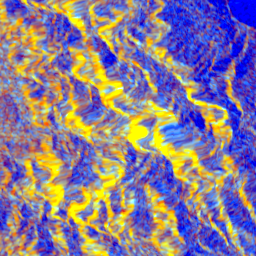
\includegraphics[width=\linewidth]{img/ROIs2017_winter_s1_68_p100.png}
    \end{subfigure}
    \begin{subfigure}{0.18\textwidth}
        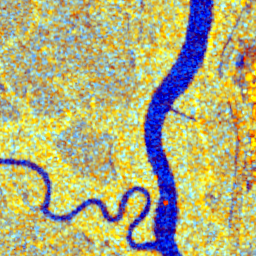
\includegraphics[width=\linewidth]{img/ROIs1970_fall_s1_105_p100.png}
    \end{subfigure}
    \begin{subfigure}{0.18\textwidth}
        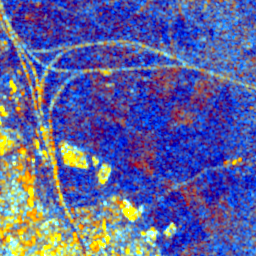
\includegraphics[width=\linewidth]{img/ROIs1970_fall_s1_128_p100.png}
    \end{subfigure}
    \begin{subfigure}{0.18\textwidth}
        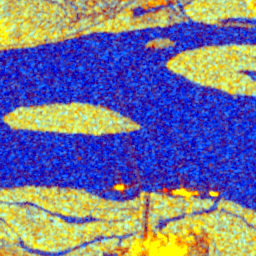
\includegraphics[width=\linewidth]{img/ROIs2017_winter_s1_104_p101.png}
    \end{subfigure}
    \begin{subfigure}{0.18\textwidth}
        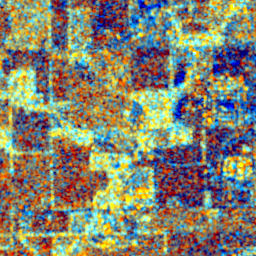
\includegraphics[width=\linewidth]{img/ROIs1970_fall_s1_145_p100.png}
    \end{subfigure}

    \begin{subfigure}{0.18\textwidth}
        \centering
        {\footnotesize \textit{Winter ROI-68-100}}
    \end{subfigure}
    \begin{subfigure}{0.18\textwidth}
        \centering
        {\footnotesize \textit{Fall ROI-105-100}}
    \end{subfigure}
    \begin{subfigure}{0.18\textwidth}
        \centering
        {\footnotesize \textit{Fall ROI-128-100}}
    \end{subfigure}
    \begin{subfigure}{0.18\textwidth}
        \centering
        {\footnotesize \textit{Winter ROI-104-101}}
    \end{subfigure}
    \begin{subfigure}{0.18\textwidth}
        \centering
        {\footnotesize \textit{Fall ROI-145-100}}
    \end{subfigure}
    
    \vspace{0.5em}

    % Second row: MS images
    \begin{subfigure}{0.18\textwidth}
        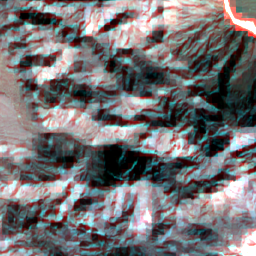
\includegraphics[width=\linewidth]{img/ROIs2017_winter_s2_68_p100.png}
    \end{subfigure}
    \begin{subfigure}{0.18\textwidth}
        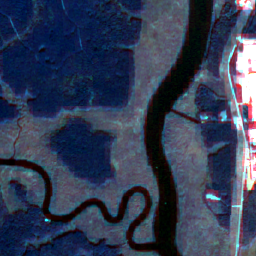
\includegraphics[width=\linewidth]{img/ROIs1970_fall_s2_105_p100.png}
    \end{subfigure}
    \begin{subfigure}{0.18\textwidth}
        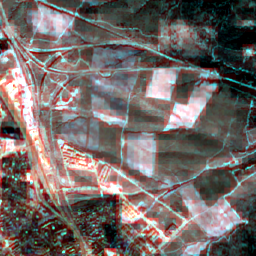
\includegraphics[width=\linewidth]{img/ROIs1970_fall_s2_128_p100.png}
    \end{subfigure}
    \begin{subfigure}{0.18\textwidth}
        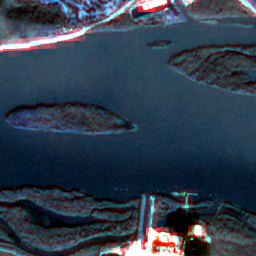
\includegraphics[width=\linewidth]{img/ROIs2017_winter_s2_104_p101.png}
    \end{subfigure}
    \begin{subfigure}{0.18\textwidth}
        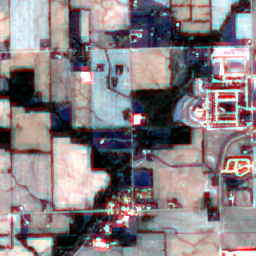
\includegraphics[width=\linewidth]{img/ROIs1970_fall_s2_145_p100.png}
    \end{subfigure}

    \caption{Sample pairs from the SEN12MS dataset. Top row: Sentinel-1 SAR patches (R: VV, G: VH, B: VV/VH). Bottom row: corresponding Sentinel-2 multispectral patches (only RGB bands).}
    \label{fig:sen12ms_pairs}
\end{figure}


Importantly, all triplets underwent manual verification by a remote sensing expert. This revision step ensured that each patch is free from major artifacts, severe registration errors, or residual cloud contamination, thereby guaranteeing the dataset’s quality and usability for machine learning tasks.

The ROIs were sampled globally across all inhabited continents and four meteorological seasons of 2017 to maximize spatial and temporal diversity. Nevertheless, it should be noted that the ROI selection was not purely random. In practice, locations were chosen to avoid large homogeneous areas such as deserts or oceans and to ensure inclusion of diverse land cover classes. While this design improves the dataset’s representativeness for a wide range of applications, it may introduce a bias toward heterogeneous landscapes and thus does not fully capture the true global distribution of land cover types.

For the purpose of this thesis, which addresses translation from SAR to multispectral optical imagery, only the Sentinel-1 and Sentinel-2 modalities are employed. The MODIS land cover products included in SEN12MS are disregarded, as they are not directly relevant to the translation task.

\subsection{SEN12 datasets Family}
SEN12MS is part of a broader line of datasets developed to foster multimodal remote sensing research. Its direct predecessor, SEN1-2~\cite{sen12_2018}, curated by the same research group, contained approximately 282,000 paired patches of Sentinel-1 VV data and Sentinel-2 RGB composites. While groundbreaking in bridging SAR and optical domains, SEN1-2 lacked georeferencing, full spectral coverage, and multi-polarization SAR, limiting its applicability for remote sensing research beyond proof-of-concept image translation.

SEN12MS addressed these limitations by introducing full multispectral coverage, dual-polarized SAR, geocoded products, and auxiliary land cover labels, making it a comprehensive multimodal benchmark. Building upon this foundation, the dataset family has since been extended. SEN12MS-CR~\cite{sen12ms-cr_2021} added temporally matched cloudy and cloud-free Sentinel-2 imagery alongside Sentinel-1 data, enabling the development and benchmarking of cloud removal methods under realistic atmospheric conditions. Subsequently, SEN12MS-CR-TS~\cite{sen12ms-cr-ts_2022} expanded the concept into the temporal domain, providing year-long multimodal time series with 30 co-registered Sentinel-1 and Sentinel-2 acquisitions per ROI. This evolution reflects a progression from simplified SAR–optical pairs, to globally diverse multimodal data, to temporally rich resources designed for time-series analysis and robust cloud removal.

A comparsion of these different datasets is provided in Table~\ref{tab:sen12_datasets}. In this thesis, however, the focus remains on the SEN12MS dataset, leveraging its multimodal SAR and multispectral imagery for the study of SAR-to-optical translation.

% in preamble:
% \usepackage{array,booktabs,adjustbox}
% ragged-right p-columns
\newcolumntype{P}[1]{>{\raggedright\arraybackslash}p{#1}}

\begin{table}[!h]
    \centering
    \caption{Comparison of datasets in the SEN12 family.}
    \label{tab:sen12_datasets}
    \setlength{\tabcolsep}{4pt} % tighter horizontal padding
    \renewcommand{\arraystretch}{1.15} % a bit more vertical room
    \begin{adjustbox}{max width=\textwidth, keepaspectratio=false}
    \begin{tabular}{P{2.6cm} P{3.4cm} P{3.4cm} P{3.6cm} P{3.6cm}}
        \toprule
        \textbf{Aspect} &
        \textbf{SEN1-2}~\cite{sen12_2018} &
        \textbf{SEN12MS}~\cite{sen12ms_2019} &
        \textbf{SEN12MS-CR}~\cite{sen12ms-cr_2021} &
        \textbf{SEN12MS-CR-TS}~\cite{sen12ms-cr-ts_2022} \\
        \midrule
        \textbf{Year released} &
        2018 & 2019 & 2021 & 2022 \\
        \addlinespace[6pt]
        \textbf{Main purpose} &
        Proof-of-concept SAR–optical translation &
        Multimodal learning and data fusion &
        Cloud removal with real cloudy/clear pairs &
        Multi-temporal cloud removal (sequence models) \\
        \addlinespace[6pt]
        \textbf{Modalities} &
        S1 (VV), S2 (RGB) &
        S1 (VV,VH), S2 (13 bands), MODIS LULC &
        S1 (VV,VH), S2 (13 bands; cloudy \& cloud-free) &
        S1 (VV,VH), S2 (13 bands; cloudy \& cloud-free time series) \\
        \addlinespace[6pt]
        \textbf{Georeferencing} &
        Not georeferenced &
        Fully georeferenced &
        Fully georeferenced &
        Fully georeferenced \\
        \addlinespace[6pt]
        \textbf{Spatial sampling} &
        Global patch pairs (282k) &
        180,662 patch triplets across 2017 seasons &
        169 ROIs; $>$100k patch triplets &
        53 ROIs; 30 time steps per ROI \\
        \addlinespace[6pt]
        \textbf{Temporal coverage} &
        Single time-point &
        Seasonal (2017) &
        Seasonal with paired cloudy/clear &
        Year-long time series (2018) \\
        \addlinespace[6pt]
        \textbf{Patch size} &
        $256\times256$ px &
        $256\times256$ px &
        $256\times256$ px &
        $256\times256$ px \\
        \addlinespace[6pt]
        \textbf{Notable limitations} &
        RGB only; VV only; no geocoding &
        MODIS labels are coarse (upsampled) &
        Mono-temporal pairs (no full time series) &
        Fewer ROIs; large storage ($\sim$2\,TB) \\
        \bottomrule
    \end{tabular}
    \end{adjustbox}
\end{table}


\section{Models}
\subsection{Pix2Pix Model}
The image translation task in this thesis is addressed using the \textit{pix2pix} framework, introduced by Isola et al.~\cite{pix2pix_2018}. Pix2pix is based on the concept of \textit{conditional generative adversarial networks} (cGANs), which extend the original GAN formulation by conditioning both the generator and discriminator on an input image. In this setup, the generator $G$ learns to map an input image $x$ to an output image $y$, while the discriminator $D$ learns to distinguish between real image pairs $\{x, y\}$ and synthesized pairs $\{x, G(x)\}$. This adversarial objective enforces that generated outputs are not only realistic but also structurally consistent with the given input.

Formally, the cGAN loss is defined as:
\begin{equation}
    \mathcal{L}_{cGAN}(G,D) = \mathbb{E}_{x,y}[\log D(x,y)] + \mathbb{E}_{x}[\log(1 - D(x,G(x)))].
\end{equation}
To encourage fidelity to the target image, the adversarial loss is combined with an $\ell_{1}$ reconstruction loss:
\begin{equation}
    \mathcal{L}_{\ell_1}(G) = \mathbb{E}_{x,y}[\|y - G(x)\|_1].
\end{equation}
The final objective is then:
\begin{equation}
    G^* = \arg \min_G \max_D \; \mathcal{L}_{cGAN}(G,D) + \lambda \mathcal{L}_{\ell_1}(G),
\end{equation}
where $\lambda$ balances realism and reconstruction accuracy. Following Isola et al., $\lambda = 100$ is typically used.

\paragraph{Generator architecture.}  
The generator is implemented as a \textit{U-Net} encoder–decoder~\cite{U-net_2015}. Unlike a plain encoder–decoder, U-Net introduces skip connections between corresponding downsampling and upsampling layers, allowing low-level spatial details from the input to directly propagate to the output. This design is particularly effective in tasks where the input and output share spatial structures, as in SAR-to-optical translation.

\paragraph{Discriminator architecture.}  
The discriminator follows a \textit{PatchGAN} design, which classifies local $N \times N$ patches of an image as real or fake instead of operating on the entire image~\cite{pix2pix_2018}. This approach emphasizes high-frequency correctness and enforces local realism, while the $\ell_1$ loss ensures global structural coherence. The original work demonstrates that a patch size of $70 \times 70$ provides a good trade-off between quality and efficiency.

\paragraph{Optimization.}  
Training alternates between updating $D$ to improve its ability to classify real versus fake pairs, and updating $G$ to fool $D$ while minimizing the $\ell_1$ distance to the target. The Adam optimizer~\cite{adam_optimizer_2017} with learning rate $2 \times 10^{-4}$ and momentum parameters $\beta_1=0.5$, $\beta_2=0.999$ is typically employed. Dropout is used at both training and inference time to introduce stochasticity, though in practice outputs remain largely deterministic.

\paragraph{Relevance to this work.}  
The pix2pix framework provides a principled and general-purpose solution for image-to-image translation tasks. In the context of this thesis, it is employed to learn mappings from Sentinel-1 SAR inputs to Sentinel-2 multispectral optical outputs. The combination of adversarial and reconstruction losses, together with the U-Net generator and PatchGAN discriminator, makes pix2pix particularly suitable for producing sharp, realistic, and structurally aligned multispectral predictions.


\section{Evaluation Metrics}
The effectiveness of SAR-to-optical image translation depends not only on the choice of translation models but also on the methods employed for quality assessment. Image Quality Assessment (IQA) serves two key purposes: (i) to objectively evaluate the quality of results produced by different models, and (ii) to guide the optimization of network architectures and algorithms~\cite{quality_assessment_S2OT}.

In~\cite{quality_assessment_S2OT}, five IQA metrics—SSIM, FSIM, MSE, LPIPS, and DISTS—were compared through image restoration experiments to identify suitable measures for SAR-to-optical translation. Their results showed that SSIM, MSE, and LPIPS consistently aligned with human perception, converged reliably, and effectively captured both structural and textural details, whereas FSIM often failed to capture fine details and DISTS exhibited instability. Consequently, SSIM, MSE, and LPIPS were recommended as complementary metrics for pixel-level fidelity, structural similarity, and perceptual quality. Nevertheless, as summarized in Table~\ref{tab:iqa}, SSIM, PSNR, and SAM remain the most widely used indicators in SAR-to-optical translation, fusion, and cloud removal tasks, while LPIPS and MSE appear far less frequently. This distribution is consistent with the findings reported in the literature survey~\cite{sar_2_opt_CGAN_survey_taxonomy}.

\textcolor{red}{TODO: specify which metrics will be used and why}

\begin{table}[h!]
\centering
\begin{tabular}{lll}
\toprule
\textbf{Metric} & \textbf{References} & \textbf{Frequency} \\
\midrule
Structural Similarity Index Measurement (SSIM)~\cite{iqa_ssim}
 & \cite{CR_Advances_Review_ORS, RS_Data_Fusion_GANs_sota, DiffCR, c_diffusion_s2o, s2o_ViT_cGAN, S2MS_GAN, c_guided_fus_s2ot, transfusion_cr, trans_gan_CF, hvt_cgan, msf_gan, diffusion_memory} 
 & 12 \\
Peak Signal-to-Noise Ratio (PSNR)~\cite{iqa_psnr}
 & \cite{CR_Advances_Review_ORS, DiffCR, CR_RS_spati_atten_GAN, s2o_ViT_cGAN, CR_RS_GAN_s2o, S2MS_GAN, c_guided_fus_s2ot, transfusion_cr, trans_gan_CF, hvt_cgan, msf_gan, diffusion_memory} 
 & 12 \\
Spectral Angle Mapper (SAM)~\cite{iqa_sam}
 & \cite{aCGAN_fuse_sar_MS, RS_Data_Fusion_GANs_sota, CR_RS_GAN_s2o, S2MS_GAN, c_guided_fus_s2ot, transfusion_cr, trans_gan_CF, cond_brownian, hvt_cgan, msf_gan} 
 & 11 \\
Fréchet Inception Distance (FID)~\cite{iqa_fid}
 & \cite{DiffCR, c_diffusion_s2o, s2o_ViT_cGAN, cond_brownian, hvt_cgan, msf_gan} 
 & 6 \\
Root Mean Square Error (RMSE) 
 & \cite{aCGAN_fuse_sar_MS, CR_Advances_Review_ORS, RS_Data_Fusion_GANs_sota, CR_RS_GAN_s2o, c_guided_fus_s2ot} 
 & 5 \\
Learned Perceptual Image Patch Similarity (LPIPS)~\cite{iqa_lpips}
 & \cite{CR_Advances_Review_ORS, DiffCR, S2MS_GAN, cond_brownian, diffusion_memory} 
 & 5 \\
Mean Absolute Error (MAE) 
 & \cite{CR_RS_GAN_s2o, c_guided_fus_s2ot} 
 & 2 \\
Mean Square Error (MSE) 
 & \cite{CR_RS_spati_atten_GAN, trans_gan_CF} 
 & 2 \\
\bottomrule
\end{tabular}
\caption{Common evaluation metrics for SAR-to-optical and cloud removal tasks.}
\label{tab:iqa}
\end{table}

\paragraph{SSIM}
The Structural Similarity Index (SSIM)~\cite{iqa_ssim} measures perceptual similarity by comparing local patterns of luminance, contrast, and structure between two images. Unlike pixel-wise errors, it models human visual sensitivity to structural distortions~\cite{DiffCR,hvt_cgan}, which is crucial for evaluating translated images. For two images $x$ and $y$, SSIM is defined as
\begin{equation}
\text{SSIM}(x,y) = \frac{(2\mu_x \mu_y + c_1)(2\sigma_{xy} + c_2)}{(\mu_x^2 + \mu_y^2 + c_1)(\sigma_x^2 + \sigma_y^2 + c_2)},
\end{equation}
where $\mu_x, \mu_y$ are means, $\sigma_x^2, \sigma_y^2$ variances, and $\sigma_{xy}$ the covariance. Values close to 1 indicate strong structural similarity. By focusing on local patterns of pixel intensities and their structural relationships, SSIM better reflects perceptual fidelity compared to raw pixel-difference metric


\paragraph{PSNR} 
The Peak Signal-to-Noise Ratio (PSNR) quantifies the distortion between a reconstructed image and its reference. PSNR is directly related to the Mean Squared Error (MSE), measuring pixel-level fidelity by comparing the residual error to the maximum possible signal intensity. For two images $x$ and $y$, PSNR is defined as
\begin{equation}
\text{PSNR}(x,y) = 10 \cdot \log_{10} \left( \frac{MAX^2}{\text{MSE}(x,y)} \right),
\end{equation}
with
\begin{equation}
\text{MSE}(x,y) = \frac{1}{N} \sum_{i=1}^{N} (x_i - y_i)^2,
\end{equation}
where $x_i$ and $y_i$ denote the pixel values of the generated and reference images, $N$ is the total number of pixels, and $MAX$ is the maximum pixel intensity (typically $255$ for 8-bit images).  

Higher PSNR values indicate lower distortion and better image quality, as they imply that the reconstructed image more closely approximates the reference. Despite its popularity for tasks such as denoising and compression, PSNR is limited by its purely pixel-wise formulation and often correlates weakly with human visual perception~\cite{DiffCR}.

\paragraph{SAM} 
The Spectral Angle Mapper (SAM), originally proposed by Kruse et al.~\cite{iqa_sam} in 1993, is widely employed in remote sensing to evaluate the spectral fidelity of reconstructed images. SAM regards the spectrum of each pixel as a high-dimensional vector and quantifies similarity by measuring the angle between the generated and reference spectral vectors. For two spectral vectors $x$ and $y$, SAM is defined as
\begin{equation}
\text{SAM}(x,y) = \arccos \left( \frac{\langle x, y \rangle}{\|x\|_2 \cdot \|y\|_2} \right),
\end{equation}
where $\langle x,y \rangle$ denotes the dot product and $\|\cdot\|_2$ is the Euclidean norm.  

SAM is typically expressed in degrees, with smaller values indicating higher spectral similarity and less distortion. Since it only considers the direction of the spectral vectors and not their magnitude, SAM is invariant to changes in illumination, making it particularly suitable for remote sensing and multispectral image analysis~\cite{S2MS_GAN}. In practice, the global SAM score is computed as the average angle across all pixels in the image.

\paragraph{LPIPS} 
The Learned Perceptual Image Patch Similarity (LPIPS) metric was proposed by Zhang et al.~\cite{iqa_lpips} to provide a perceptual measure of image similarity that better aligns with human visual judgment. It compares feature activations from pretrained convolutional networks, thereby capturing high-level semantics and perceptual realism. For two images $x$ and $y$, LPIPS is defined as
\begin{equation}
\text{LPIPS}(x,y) = \sum_{l} w_l \cdot \| f_l(x) - f_l(y) \|_2,
\end{equation}
where $f_l(\cdot)$ denotes the feature representation in the $l$-th layer of the network and $w_l$ is a learned weight.  

By measuring differences in a deep feature space rather than raw pixel intensities, LPIPS reflects perceptual similarity and visual realism. Lower LPIPS values indicate that the generated image is closer to the reference in terms of human-perceived quality~\cite{CR_Advances_Review_ORS,DiffCR}, making this metric particularly useful for evaluating the naturalness of translated images.

\paragraph{FID} 
Introduced in 2018 by Heusel at el.~\cite{iqa_fid}, the Fréchet Inception Distance (FID) is a perceptual metric that evaluates the realism of generated images at the distributional level. Instead of comparing images pixel by pixel, FID measures the distance between the feature distributions of generated and reference images, extracted by a pretrained Inception network. Let $(\mu_r, \Sigma_r)$ and $(\mu_g, \Sigma_g)$ denote the mean and covariance of the reference and generated feature distributions, respectively. FID is defined as
\begin{equation}
\text{FID} = \| \mu_r - \mu_g \|_2^2 + \text{Tr}\left( \Sigma_r + \Sigma_g - 2(\Sigma_r \Sigma_g)^{1/2} \right).
\end{equation}

Lower FID values indicate closer alignment between generated and real image distributions. While LPIPS assesses pairwise perceptual similarity, FID captures distributional alignment, making the two metrics complementary.


\paragraph{Evaluation Protocol}
The evaluation of SAR-to-optical translation performance was conducted using PSNR, SSIM, and SAM, complemented by a perceptual metric (LPIPS or FID). PSNR quantifies pixel-level fidelity, SSIM assesses local structural similarity, and SAM measures spectral consistency across all bands, which is critical in multispectral applications. To additionally capture perceptual realism beyond pixel-wise statistics, a deep feature–based perceptual score was employed, with LPIPS enabling pairwise comparisons and FID providing distributional similarity. For outputs with more than three bands, perceptual metrics were computed on a fixed RGB composite for both reference and prediction, and this limitation was explicitly acknowledged. This combination of metrics provides a comprehensive assessment covering spatial fidelity, structural integrity, spectral accuracy, and perceptual quality.

\begin{table}[h!]
	\centering
	\caption{Summary of evaluation metrics for SAR-to-multispectral translation.}
	\begin{tabularx}{\textwidth}{p{1.7cm}X X X}
		\toprule 
		\textbf{Metric} & \textbf{Aspect Evaluated} & \textbf{Advantages} & \textbf{Limitations} \\
		\midrule 
		PSNR  & Pixel-level fidelity via mean squared error ratio & Simple, widely used, interpretable in terms of noise/distortion & Correlates weakly with human perception; sensitive to pixel shifts \\
		SSIM  & Structural similarity (luminance, contrast, texture) & Captures perceptual structure better than PSNR; patch-based & Still intensity-based; limited correlation with perceptual realism \\
		SAM   & Spectral fidelity across bands & Invariant to illumination; critical for multispectral data integrity & Ignores spatial/structural context; only reflects spectral angle \\
		LPIPS & Perceptual similarity using deep features (pairwise) & Aligns well with human judgment; sensitive to high-level semantics & Requires pretrained CNN; limited to 3-channel inputs unless adapted \\
		FID   & Distributional similarity in feature space & Evaluates realism of entire image sets; widely adopted in generative models & Requires large sample size; sensitive to preprocessing; assumes Gaussian feature distributions \\
		\bottomrule
	\end{tabularx}
\end{table}

\chapter{Experiments}

\begin{table}[]
\centering
\caption{Data cropped to 64x64, channels kept raw}
\label{tab:experiment_results}
\begin{tabular}{lcccc}
\hline
\textbf{Model} & \textbf{MAE} $\downarrow$ & \textbf{RMSE} $\downarrow$ & \textbf{PSNR (dB)} $\uparrow$ & \textbf{SSIM} $\uparrow$ \\
\hline
pix2pix  & 68.06 & 291.62 & 37.54 & 0.9545 \\
SwinUnet & 41.58 & 181.62 & 41.11 & 0.9687 \\
UMamba   & 35.14 & 158.47 & 42.67 & 0.9757 \\
SiMaVP   & \textbf{31.41} & \textbf{139.95} & \textbf{43.75} & \textbf{0.9797} \\
\hline
\end{tabular}
\end{table}


\chapter{Discussion}

\chapter{Conclusion}



\bibliographystyle{IEEEtran}
\bibliography{references}

\nocite{*}
\end{document}
